%% template.tex
%% from
%% bare_conf.tex
%% V1.4b
%% 2015/08/26
%% by Michael Shell
%% See:
%% http://www.michaelshell.org/
%% for current contact information.
%%
%% This is a skeleton file demonstrating the use of IEEEtran.cls
%% (requires IEEEtran.cls version 1.8b or later) with an IEEE
%% conference paper.
%%
%% Support sites:
%% http://www.michaelshell.org/tex/ieeetran/
%% http://www.ctan.org/pkg/ieeetran
%% and
%% http://www.ieee.org/

%%*************************************************************************
%% Legal Notice:
%% This code is offered as-is without any warranty either expressed or
%% implied; without even the implied warranty of MERCHANTABILITY or
%% FITNESS FOR A PARTICULAR PURPOSE!
%% User assumes all risk.
%% In no event shall the IEEE or any contributor to this code be liable for
%% any damages or losses, including, but not limited to, incidental,
%% consequential, or any other damages, resulting from the use or misuse
%% of any information contained here.
%%
%% All comments are the opinions of their respective authors and are not
%% necessarily endorsed by the IEEE.
%%
%% This work is distributed under the LaTeX Project Public License (LPPL)
%% ( http://www.latex-project.org/ ) version 1.3, and may be freely used,
%% distributed and modified. A copy of the LPPL, version 1.3, is included
%% in the base LaTeX documentation of all distributions of LaTeX released
%% 2003/12/01 or later.
%% Retain all contribution notices and credits.
%% ** Modified files should be clearly indicated as such, including  **
%% ** renaming them and changing author support contact information. **
%%*************************************************************************


% *** Authors should verify (and, if needed, correct) their LaTeX system  ***
% *** with the testflow diagnostic prior to trusting their LaTeX platform ***
% *** with production work. The IEEE's font choices and paper sizes can   ***
% *** trigger bugs that do not appear when using other class files.       ***                          ***
% The testflow support page is at:
% http://www.michaelshell.org/tex/testflow/

\documentclass[conference,final,]{IEEEtran}
% Some Computer Society conferences also require the compsoc mode option,
% but others use the standard conference format.
%
% If IEEEtran.cls has not been installed into the LaTeX system files,
% manually specify the path to it like:
% \documentclass[conference]{../sty/IEEEtran}





% Some very useful LaTeX packages include:
% (uncomment the ones you want to load)


% *** MISC UTILITY PACKAGES ***
%
%\usepackage{ifpdf}
% Heiko Oberdiek's ifpdf.sty is very useful if you need conditional
% compilation based on whether the output is pdf or dvi.
% usage:
% \ifpdf
%   % pdf code
% \else
%   % dvi code
% \fi
% The latest version of ifpdf.sty can be obtained from:
% http://www.ctan.org/pkg/ifpdf
% Also, note that IEEEtran.cls V1.7 and later provides a builtin
% \ifCLASSINFOpdf conditional that works the same way.
% When switching from latex to pdflatex and vice-versa, the compiler may
% have to be run twice to clear warning/error messages.






% *** CITATION PACKAGES ***
%
%\usepackage{cite}
% cite.sty was written by Donald Arseneau
% V1.6 and later of IEEEtran pre-defines the format of the cite.sty package
% \cite{} output to follow that of the IEEE. Loading the cite package will
% result in citation numbers being automatically sorted and properly
% "compressed/ranged". e.g., [1], [9], [2], [7], [5], [6] without using
% cite.sty will become [1], [2], [5]--[7], [9] using cite.sty. cite.sty's
% \cite will automatically add leading space, if needed. Use cite.sty's
% noadjust option (cite.sty V3.8 and later) if you want to turn this off
% such as if a citation ever needs to be enclosed in parenthesis.
% cite.sty is already installed on most LaTeX systems. Be sure and use
% version 5.0 (2009-03-20) and later if using hyperref.sty.
% The latest version can be obtained at:
% http://www.ctan.org/pkg/cite
% The documentation is contained in the cite.sty file itself.






% *** GRAPHICS RELATED PACKAGES ***
%
\ifCLASSINFOpdf
  % \usepackage[pdftex]{graphicx}
  % declare the path(s) where your graphic files are
  % \graphicspath{{../pdf/}{../jpeg/}}
  % and their extensions so you won't have to specify these with
  % every instance of \includegraphics
  % \DeclareGraphicsExtensions{.pdf,.jpeg,.png}
\else
  % or other class option (dvipsone, dvipdf, if not using dvips). graphicx
  % will default to the driver specified in the system graphics.cfg if no
  % driver is specified.
  % \usepackage[dvips]{graphicx}
  % declare the path(s) where your graphic files are
  % \graphicspath{{../eps/}}
  % and their extensions so you won't have to specify these with
  % every instance of \includegraphics
  % \DeclareGraphicsExtensions{.eps}
\fi
% graphicx was written by David Carlisle and Sebastian Rahtz. It is
% required if you want graphics, photos, etc. graphicx.sty is already
% installed on most LaTeX systems. The latest version and documentation
% can be obtained at:
% http://www.ctan.org/pkg/graphicx
% Another good source of documentation is "Using Imported Graphics in
% LaTeX2e" by Keith Reckdahl which can be found at:
% http://www.ctan.org/pkg/epslatex
%
% latex, and pdflatex in dvi mode, support graphics in encapsulated
% postscript (.eps) format. pdflatex in pdf mode supports graphics
% in .pdf, .jpeg, .png and .mps (metapost) formats. Users should ensure
% that all non-photo figures use a vector format (.eps, .pdf, .mps) and
% not a bitmapped formats (.jpeg, .png). The IEEE frowns on bitmapped formats
% which can result in "jaggedy"/blurry rendering of lines and letters as
% well as large increases in file sizes.
%
% You can find documentation about the pdfTeX application at:
% http://www.tug.org/applications/pdftex

\usepackage{graphicx}

% *** MATH PACKAGES ***
%
\usepackage{amsmath}
\interdisplaylinepenalty=2500
%\usepackage{amsmath}
% A popular package from the American Mathematical Society that provides
% many useful and powerful commands for dealing with mathematics.
%
% Note that the amsmath package sets \interdisplaylinepenalty to 10000
% thus preventing page breaks from occurring within multiline equations. Use:
%\interdisplaylinepenalty=2500
% after loading amsmath to restore such page breaks as IEEEtran.cls normally
% does. amsmath.sty is already installed on most LaTeX systems. The latest
% version and documentation can be obtained at:
% http://www.ctan.org/pkg/amsmath





% *** SPECIALIZED LIST PACKAGES ***
%
%\usepackage{algorithmic}
% algorithmic.sty was written by Peter Williams and Rogerio Brito.
% This package provides an algorithmic environment fo describing algorithms.
% You can use the algorithmic environment in-text or within a figure
% environment to provide for a floating algorithm. Do NOT use the algorithm
% floating environment provided by algorithm.sty (by the same authors) or
% algorithm2e.sty (by Christophe Fiorio) as the IEEE does not use dedicated
% algorithm float types and packages that provide these will not provide
% correct IEEE style captions. The latest version and documentation of
% algorithmic.sty can be obtained at:
% http://www.ctan.org/pkg/algorithms
% Also of interest may be the (relatively newer and more customizable)
% algorithmicx.sty package by Szasz Janos:
% http://www.ctan.org/pkg/algorithmicx




% *** ALIGNMENT PACKAGES ***
%
%\usepackage{array}
% Frank Mittelbach's and David Carlisle's array.sty patches and improves
% the standard LaTeX2e array and tabular environments to provide better
% appearance and additional user controls. As the default LaTeX2e table
% generation code is lacking to the point of almost being broken with
% respect to the quality of the end results, all users are strongly
% advised to use an enhanced (at the very least that provided by array.sty)
% set of table tools. array.sty is already installed on most systems. The
% latest version and documentation can be obtained at:
% http://www.ctan.org/pkg/array


% IEEEtran contains the IEEEeqnarray family of commands that can be used to
% generate multiline equations as well as matrices, tables, etc., of high
% quality.




% *** SUBFIGURE PACKAGES ***
%\ifCLASSOPTIONcompsoc
%  \usepackage[caption=false,font=normalsize,labelfont=sf,textfont=sf]{subfig}
%\else
%  \usepackage[caption=false,font=footnotesize]{subfig}
%\fi
% subfig.sty, written by Steven Douglas Cochran, is the modern replacement
% for subfigure.sty, the latter of which is no longer maintained and is
% incompatible with some LaTeX packages including fixltx2e. However,
% subfig.sty requires and automatically loads Axel Sommerfeldt's caption.sty
% which will override IEEEtran.cls' handling of captions and this will result
% in non-IEEE style figure/table captions. To prevent this problem, be sure
% and invoke subfig.sty's "caption=false" package option (available since
% subfig.sty version 1.3, 2005/06/28) as this is will preserve IEEEtran.cls
% handling of captions.
% Note that the Computer Society format requires a larger sans serif font
% than the serif footnote size font used in traditional IEEE formatting
% and thus the need to invoke different subfig.sty package options depending
% on whether compsoc mode has been enabled.
%
% The latest version and documentation of subfig.sty can be obtained at:
% http://www.ctan.org/pkg/subfig




% *** FLOAT PACKAGES ***
%

%\usepackage{fixltx2e}
% fixltx2e, the successor to the earlier fix2col.sty, was written by
% Frank Mittelbach and David Carlisle. This package corrects a few problems
% in the LaTeX2e kernel, the most notable of which is that in current
% LaTeX2e releases, the ordering of single and double column floats is not
% guaranteed to be preserved. Thus, an unpatched LaTeX2e can allow a
% single column figure to be placed prior to an earlier double column
% figure.
% Be aware that LaTeX2e kernels dated 2015 and later have fixltx2e.sty's
% corrections already built into the system in which case a warning will
% be issued if an attempt is made to load fixltx2e.sty as it is no longer
% needed.
% The latest version and documentation can be found at:
% http://www.ctan.org/pkg/fixltx2e


%\usepackage{stfloats}
% stfloats.sty was written by Sigitas Tolusis. This package gives LaTeX2e
% the ability to do double column floats at the bottom of the page as well
% as the top. (e.g., "\begin{figure*}[!b]" is not normally possible in
% LaTeX2e). It also provides a command:
%\fnbelowfloat
% to enable the placement of footnotes below bottom floats (the standard
% LaTeX2e kernel puts them above bottom floats). This is an invasive package
% which rewrites many portions of the LaTeX2e float routines. It may not work
% with other packages that modify the LaTeX2e float routines. The latest
% version and documentation can be obtained at:
% http://www.ctan.org/pkg/stfloats
% Do not use the stfloats baselinefloat ability as the IEEE does not allow
% \baselineskip to stretch. Authors submitting work to the IEEE should note
% that the IEEE rarely uses double column equations and that authors should try
% to avoid such use. Do not be tempted to use the cuted.sty or midfloat.sty
% packages (also by Sigitas Tolusis) as the IEEE does not format its papers in
% such ways.
% Do not attempt to use stfloats with fixltx2e as they are incompatible.
% Instead, use Morten Hogholm'a dblfloatfix which combines the features
% of both fixltx2e and stfloats:
%
% \usepackage{dblfloatfix}
% The latest version can be found at:
% http://www.ctan.org/pkg/dblfloatfix




% *** PDF, URL AND HYPERLINK PACKAGES ***
%
%\usepackage{url}
% url.sty was written by Donald Arseneau. It provides better support for
% handling and breaking URLs. url.sty is already installed on most LaTeX
% systems. The latest version and documentation can be obtained at:
% http://www.ctan.org/pkg/url
% Basically, \url{my_url_here}.




% *** Do not adjust lengths that control margins, column widths, etc. ***
% *** Do not use packages that alter fonts (such as pslatex).         ***
% There should be no need to do such things with IEEEtran.cls V1.6 and later.
% (Unless specifically asked to do so by the journal or conference you plan
% to submit to, of course. )



%% BEGIN MY ADDITIONS %%


\usepackage[unicode=true]{hyperref}

\hypersetup{
            pdftitle={Comparing job accessibility in diverse spatial patterns in the Greater Golden Horseshoe area, Ontario, Canada},
            pdfkeywords={Job Accessibility, Spatial
Patterns, Transportation Modes, Greater Golden Horseshoe, Urban
Planning},
            pdfborder={0 0 0},
            breaklinks=true}
\urlstyle{same}  % don't use monospace font for urls

% Pandoc toggle for numbering sections (defaults to be off)
\setcounter{secnumdepth}{0}


% tightlist command for lists without linebreak
\providecommand{\tightlist}{%
  \setlength{\itemsep}{0pt}\setlength{\parskip}{0pt}}

% From pandoc table feature
\usepackage{longtable,booktabs,array}
\usepackage{calc} % for calculating minipage widths
% Correct order of tables after \paragraph or \subparagraph
\usepackage{etoolbox}
\makeatletter
\patchcmd\longtable{\par}{\if@noskipsec\mbox{}\fi\par}{}{}
\makeatother
% Allow footnotes in longtable head/foot
\IfFileExists{footnotehyper.sty}{\usepackage{footnotehyper}}{\usepackage{footnote}}
\makesavenoteenv{longtable}

% Pandoc citation processing
\newlength{\cslhangindent}
\setlength{\cslhangindent}{1.5em}
\newlength{\csllabelwidth}
\setlength{\csllabelwidth}{3em}
\newlength{\cslentryspacingunit} % times entry-spacing
\setlength{\cslentryspacingunit}{\parskip}
% for Pandoc 2.8 to 2.10.1
\newenvironment{cslreferences}%
  {}%
  {\par}
% For Pandoc 2.11+
\newenvironment{CSLReferences}[2] % #1 hanging-ident, #2 entry spacing
 {% don't indent paragraphs
  \setlength{\parindent}{0pt}
  % turn on hanging indent if param 1 is 1
  \ifodd #1
  \let\oldpar\par
  \def\par{\hangindent=\cslhangindent\oldpar}
  \fi
  % set entry spacing
  \setlength{\parskip}{#2\cslentryspacingunit}
 }%
 {}
\usepackage{calc}
\newcommand{\CSLBlock}[1]{#1\hfill\break}
\newcommand{\CSLLeftMargin}[1]{\parbox[t]{\csllabelwidth}{#1}}
\newcommand{\CSLRightInline}[1]{\parbox[t]{\linewidth - \csllabelwidth}{#1}\break}
\newcommand{\CSLIndent}[1]{\hspace{\cslhangindent}#1}


%% END MY ADDITIONS %%


\hyphenation{op-tical net-works semi-conduc-tor}

\begin{document}
%
% paper title
% Titles are generally capitalized except for words such as a, an, and, as,
% at, but, by, for, in, nor, of, on, or, the, to and up, which are usually
% not capitalized unless they are the first or last word of the title.
% Linebreaks \\ can be used within to get better formatting as desired.
% Do not put math or special symbols in the title.
\title{Comparing job accessibility in diverse spatial patterns in the
Greater Golden Horseshoe area, Ontario, Canada}

% author names and affiliations
% use a multiple column layout for up to three different
% affiliations

\author{

%% ---- classic IEEETrans wide authors' list ----------------
\IEEEauthorblockN{
Bruno Dias dos Santos\IEEEauthorrefmark{1}%%
}

\IEEEauthorblockA{\IEEEauthorrefmark{1}
School of Earth, Environment and Society (SEES)\\
Georgia Institute of Technology,
1280 Main Street West, Hamilton, Ontario, Canada, L8S 4K1
\\ dossanb@mcmaster.ca
}

%% ----------------------------------------------------------

%% ---- classic IEEETrans one column per institution --------
 %%
%% ----------------------------------------------------------





%% ---- one column per author, classic/default IEEETrans ----

%% ----------------------------------------------------------

}

% conference papers do not typically use \thanks and this command
% is locked out in conference mode. If really needed, such as for
% the acknowledgment of grants, issue a \IEEEoverridecommandlockouts
% after \documentclass

% for over three affiliations, or if they all won't fit within the width
% of the page, use this alternative format:
%
%\author{\IEEEauthorblockN{Michael Shell\IEEEauthorrefmark{1},
%Homer Simpson\IEEEauthorrefmark{2},
%James Kirk\IEEEauthorrefmark{3},
%Montgomery Scott\IEEEauthorrefmark{3} and
%Eldon Tyrell\IEEEauthorrefmark{4}}
%\IEEEauthorblockA{\IEEEauthorrefmark{1}School of Electrical and Computer Engineering\\
%Georgia Institute of Technology,
%Atlanta, Georgia 30332--0250\\ Email: see http://www.michaelshell.org/contact.html}
%\IEEEauthorblockA{\IEEEauthorrefmark{2}Twentieth Century Fox, Springfield, USA\\
%Email: homer@thesimpsons.com}
%\IEEEauthorblockA{\IEEEauthorrefmark{3}Starfleet Academy, San Francisco, California 96678-2391\\
%Telephone: (800) 555--1212, Fax: (888) 555--1212}
%\IEEEauthorblockA{\IEEEauthorrefmark{4}Tyrell Inc., 123 Replicant Street, Los Angeles, California 90210--4321}}




% use for special paper notices
%\IEEEspecialpapernotice{(Invited Paper)}




% make the title area
\maketitle

% As a general rule, do not put math, special symbols or citations
% in the abstract
\begin{abstract}
This work aims to analyze job accessibility across diverse spatial
patterns in the Greater Golden Horseshoe area, Ontario, Canada. Using
variables extracted from satellite images, we identified six distinct
spatial patterns with variations in building density, land use, and
street layout. Afterwards, we compared accessibility to employment
considering different modes of transportation in the identified spatial
patterns. Results show that higher building density spatial patterns
exhibit elevated accessibility for all transportation modes. The job
accessibility is concentrated in approximately 10\% of the GGH, posing
challenges for spatial planners to devise a transportation system that
accommodates these territorial differences. Statistical analyses confirm
significant differences in job accessibility among spatial patterns.
\end{abstract}

% keywords
\begin{IEEEkeywords}
Job Accessibility; Spatial Patterns; Transportation Modes; Greater
Golden Horseshoe; Urban Planning
\end{IEEEkeywords}

% use for special paper notices



% make the title area
\maketitle

% no keywords

% For peer review papers, you can put extra information on the cover
% page as needed:
% \ifCLASSOPTIONpeerreview
% \begin{center} \bfseries EDICS Category: 3-BBND \end{center}
% \fi
%
% For peerreview papers, this IEEEtran command inserts a page break and
% creates the second title. It will be ignored for other modes.
\IEEEpeerreviewmaketitle


\hypertarget{introduction}{%
\section{Introduction}\label{introduction}}

Accessibility is defined as the potential to reach spatially distributed
places and opportunities (Páez et al., 2012), such as jobs, parks,
cultural activities, health, and education services. The accessibility
to these diverse opportunities is directly dependent on the
transportation network and the geographical distribution of activities,
making it a key output of spatial planning.

A survey conducted by Palm et al. (2023) revealed that labor force
participation ranks among the top five most compelling topics for
expanding the applications of accessibility studies . The survey
included over 50 participants from five Canadian provinces, with half
representing the government, the majority of whom were employed in local
government. Job accessibility serves as a crucial tool for comprehending
urban form, the spatial mismatch between jobs and housing, and the
balance between job and housing locations.

With the general context presented, this work is guided by the following
question: How does job accessibility levels vary considering diverse
spatial patterns? We posit the following hypothesis: job accessibility
differs among various spatial patterns, even when different
transportation modes are considered. The primary objective of this study
is to analyze and compare job accessibility levels across different
spatial patterns, focusing on the Greater Golden Horseshoe area (GGH) in
Ontario, Canada. We compared the transportation modes: walking, cycling,
public transportation off peak and on peak.

\hypertarget{study-area}{%
\section{Study area}\label{study-area}}

The Greater Golden Horseshoe (GGH) constitutes the urban region centered
around the City of Toronto, positioned at the western terminus of Lake
Ontario (Figure \ref{fig:GGH}). It extends northward to Georgian Bay,
southward to Lake Erie, westward to Wellington County and Waterloo
Region, and eastward to the counties of Peterborough and Northumberland.
With a population of 10 million people and accommodating 4.9 million
jobs in an area of 26,804 km², the GGH serves as the economic hub of
Ontario and stands out as one of the rapidly advancing regions in North
America (Ontario, 2020).

\begin{figure}[!t]
\centering
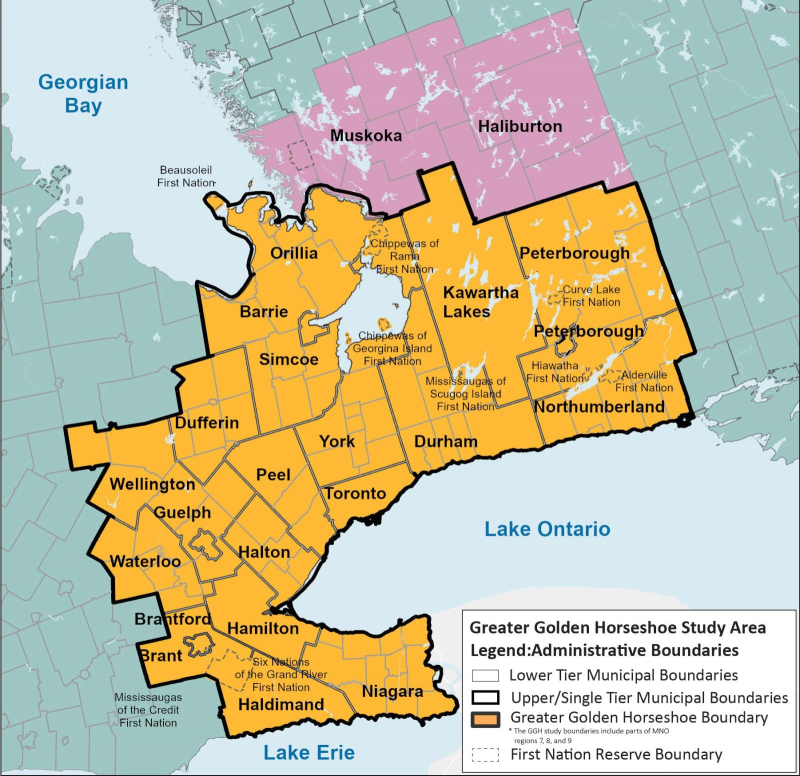
\includegraphics[width=3.5in]{C:/Users/brdia/Desktop/RSAccess/figures/mto-map-ggh-study-area-en-800x776-2022-01-31.png}
\caption{Greater Golden Horseshoe Study Area. Source: Ontario, 2020.}
\label{fig:GGH}
\end{figure}

\hypertarget{methods}{%
\section{Methods}\label{methods}}

Our methodology comprises four primary steps. The initial step involves
feature extraction and dataset creation, where urban form attributes are
extracted from satellite imagery and road network data, subsequently
mapped onto a hexagonal grid. The second step employs Principal
Component Analysis (PCA) to reduce dataset dimensionality. Utilizing
only the principal components, we conduct a non-supervised
classification to identify clusters representing the distinct spatial
patterns within the GGH. In the final step, we compare job accessibility
levels among the identified spatial patterns. Two statistical tests, the
Kruskal-Wallis test and the pairwise Wilcoxon test, are employed to
evaluate variations in job accessibility levels. For this work, we used
already processed and classified satellite images provided by the Global
Human Settlement Layer (GHSL) (European Commission. Joint Research
Centre., 2023) and the Copernicus Global Land Service (CGLS) (Buchhorn
et al., n.d.); Spatial Access Measures (SAM) dataset (Statistics Canada,
n.d.), which measures accessibility to different opportunities,
considering different modes of transportation; and a road network
(OpenStreetMap, 2023) - more information about the data can be seen in
the appendix.

\hypertarget{feature-extraction}{%
\subsection{Feature extraction}\label{feature-extraction}}

We integrate the selected datasets onto a hexagonal grid with an area of
500 m², comprising 53,609 regular cells across the study area. These
hexagons served as spatial units of analysis, providing a standardized
reference for merging data from disparate sources, including the road
network and remotely sensed imagery.

For each hexagon, we extracted statistical measures --- mean, maximum,
minimum, standard deviation, median, sum, and majority values --- for
the GHSL and CGLS images. For the road network, we computed road
sinuosity and extracted road network attributes, such as the total
number of roads, intersections, intersection density (intersections per
road), and statistical values related to road sinuosity.

Additionally, spatial variables were generated through neighborhood
connections between hexagons. For each variable \("i"\), we computed the
neighbor mean value \((NM\_i)\) and the normalized difference
\((DNM\_i)\) between each hexagon and its neighborhood mean. The
methodology employed for deriving these neighborhood variables was
devised by Dos Santos et al. (2022) , utilizing a distance matrix to
identify neighboring cells within the grid. In total, 191 attributes
were extracted for each hexagonal cell.

\hypertarget{reducing-data-dimension}{%
\subsection{Reducing data dimension}\label{reducing-data-dimension}}

Understanding intraurban differences is crucial for comprehending
variations in accessibility levels. With the dataset at hand, we
selected cells based on a threshold value for the presence of built-up
areas. Hexagons with less than 10\% of the sum of residential and
commercial buildings were excluded from the analysis. This criterion was
implemented to enhance the clustering process. Without this restriction,
the clustering algorithm tended to create numerous clusters outside the
urban area, without showing the intraurban differences.

We employed Principal Component Analysis (PCA) to reduce the
dimensionality of the data. PCA is a technique used to select features
and decrease dimensions in the presence of multiple variables. It
achieves this by generating a reduced number of linear combinations of
the original variables while preserving a substantial amount of the
information contained in them (Ringnér, 2008) . We retained all
components where the cumulative variance explained accounted for more
than 90\% of the total variance in the data. Subsequently, we
standardized the components into Z-scores for the application of PCA.

\hypertarget{identifying-spatial-patterns}{%
\subsection{Identifying spatial
patterns}\label{identifying-spatial-patterns}}

Using only the selected components, we applied an unsupervised
classification with the K-mean algorithm to identify the spatial
patterns of GGH. K-Means is a clustering algorithm, which takes as input
a number k of clusters and the algorithm divides the instances into k
clusters. The algorithm optimizes the separation between the groups by
minimizing the internal variation of the clusters - the inertia. The
clustering process is accelerated by randomly assigning the instances to
one of the k clusters and then redistributing the instances in order to
reduce the distance (in our case, the Euclidian distance) between each
observation and the central point (the centroid) of its cluster.

\hypertarget{evaluating-job-accessibility}{%
\subsection{Evaluating job
accessibility}\label{evaluating-job-accessibility}}

We transferred the SAM data from the dissemination blocks to the cell
grid using a weighted area interpolation. This technique enables us to
disaggregate accessibility values to another spatial unit, smoothing
variations between polygons. It achieves this by using the area of
overlapping geometries to apportion variables.

Following this, we conducted an initial statistical test to assess job
accessibility levels across spatial patterns. Given that the job
accessibility variables did not exhibit a normal distribution, we
employed the Kruskal-Wallis test to determine whether the accessibility
medians differed among the clusters. If a median difference was
identified between the groups, we then applied the pairwise Wilcoxon
test to discern which specific group differed from the others. We
adopted a significance level of 0.05 for both tests.

\hypertarget{results}{%
\section{Results}\label{results}}

\hypertarget{principal-components-analysis}{%
\subsection{Principal Components
Analysis}\label{principal-components-analysis}}

For the clustering analysis, thirty-five principal components were
selected, collectively explaining over 90\% of the total variance. Table
\ref{tab:loading-table} highlights the three most significant variable
contributions to the first four principal components. Across all
components, variables related to neighbor relations demonstrated the
most substantial loadings. Component 1 exhibits higher absolute loadings
in the neighbor mean of built-up type variables, predominantly
associated with more densely built-up areas in the study area; Component
2 displays higher absolute loadings in variables related to the fraction
of water on neighboring cells, indicating a correlation with waterfront
areas; Component 3 focuses on the presence of built-up areas and
residential use in neighboring cells; and Component 4 correlates with
the presence of trees in neighboring cells.

\begin{table}[!hb]
\centering
\caption{HIGHER VARIABLES CONTRIBUTIONS TO THE FIRST FOUR PRINCIPAL
COMPONENTES (PC)}
\label{tab:loading-table}
\resizebox{\columnwidth}{!}{%
\begin{tabular}{@{}lcccc@{}}
\toprule
\textbf{Variable}      & \textbf{PC1}   & \textbf{PC2}  & \textbf{PC3}   & \textbf{PC4}   \\ \midrule
Built-up sum (NM)      & \textbf{0.12}  & -0.03         & -0.03          & 0.02           \\
Built-up mean (NM)     & \textbf{0.12}  & -0.03         & -0.03          & 0.02           \\
Comercial area (NM)    & \textbf{-0.11} & 0.02          & 0.01           & -0.03          \\
Water mean (NM)        & -0.01          & \textbf{0.19} & -0.02          & -0.11          \\
Water sum (NM)         & -0.01          & \textbf{0.19} & -0.02          & -0.11          \\
Water median (NM)      & -0.01          & \textbf{0.19} & -0.03          & -0.11          \\
Built-up mean (DNM)    & -0.06          & 0.03          & \textbf{-0.23} & 0.04           \\
Built-up sum (DNM)     & -0.06          & 0.03          & \textbf{-0.23} & 0.04           \\
Residential area (DNM) & -0.06          & 0.02          & \textbf{-0.23} & 0.03           \\
Tree mean (DNM)        & 0.07           & -0.04         & 0.05           & \textbf{-0.16} \\
Tree sum (DNM)         & 0.07           & -0.04         & 0.05           & \textbf{-0.16} \\
Tree median (DNM)      & 0.06           & -0.03         & 0.02           & \textbf{-0.16} \\ \midrule
Proportion of Variance & 35\%           & 9\%           & 6\%            & 5\%            \\
Cumulative Proportion  & 35\%           & 45\%          & 51\%           & 56\%           \\ \bottomrule
\end{tabular}%
}
\end{table}

\hypertarget{clustering-result}{%
\subsection{Clustering result}\label{clustering-result}}

Only one-quarter of the study area was analyzed to perform the
clustering classification, as only these cells had the sum of
residential and commercial areas exceeding ten percent of the cell area.
A series of experiments and visual analyses were conducted to determine
the optimal number of clusters. After several experiments and visual
analyses, we settled on six final clusters, considering the best
trade-off between identifying meaningful clusters and their quantity
(Figure \ref{fig:clusters_map}).

\begin{figure}[!bt]
\centering
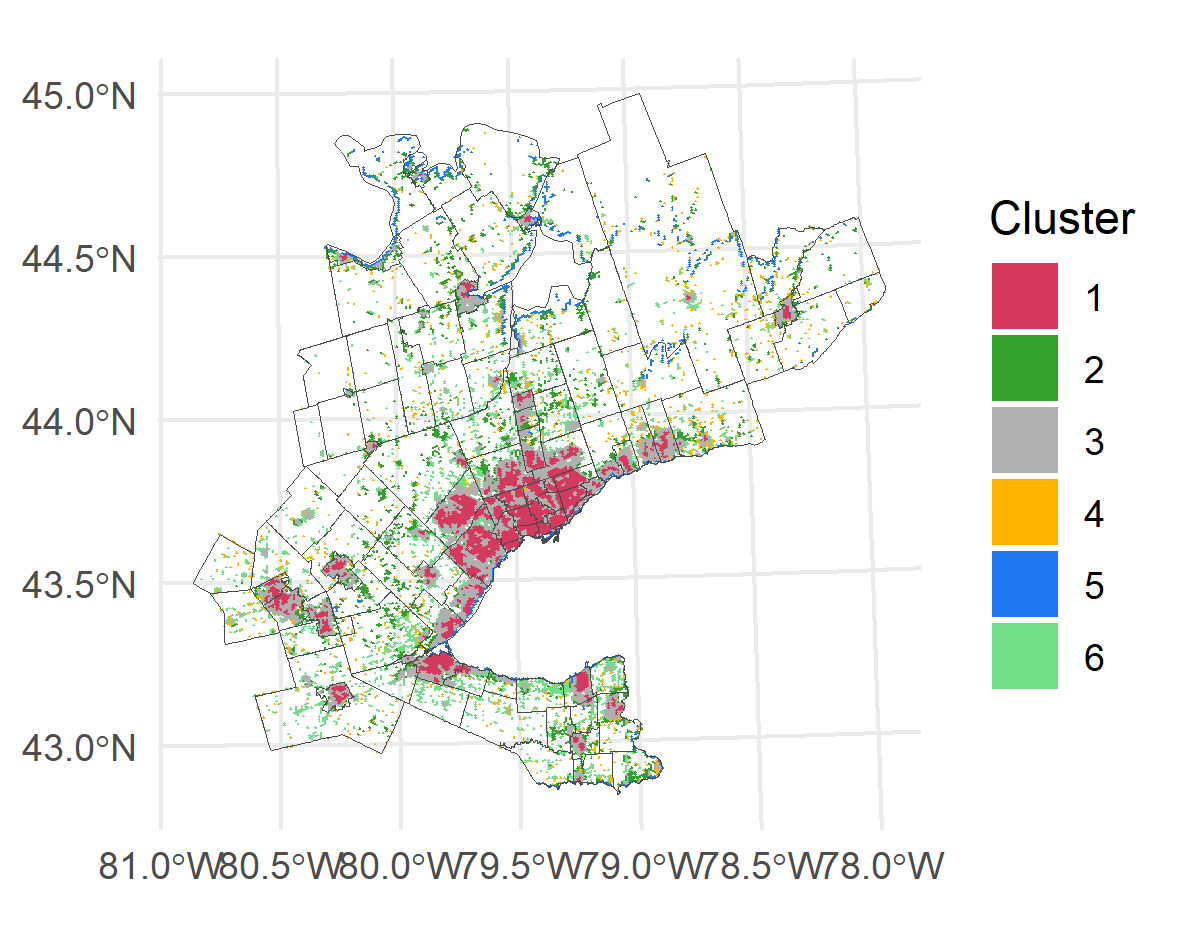
\includegraphics[width=3.5in]{C:/Users/brdia/Desktop/RSAccess/figures/spatial_patterns_map.png}
\caption{Study area spatial patterns.}
\label{fig:clusters_map}
\end{figure}

Each final cluster can be interpreted as a distinct spatial pattern with
unique levels of built-up area density, land use, and street layout. We
named the spatial patterns according to their features. The first
cluster, ``Cluster 1 - High Building Density,'' corresponds to 17\% of
the analyzed clusters and exhibits the highest building density (in
area, height, and volume) among all clusters. It also has the highest
number of intersections per road, suggesting more connections between
its streets. In turn, ``Cluster 2 - Tree-lined Neighborhoods'' is mainly
characterized by the highest presence of trees, with about 20\% of its
area dedicated to residential use, no commercial areas, and a low
inclination for farms. Eighteen percent of the clusters belong to this
class, located at the periphery of urban areas. The third cluster,
``Cluster 3 - Medium Building Density,'' is the largest, accounting for
28\% of the analyzed area. Situated at the border of the first clusters,
it features the second most residential and commercial areas. ``Cluster
4 - Mixed Rural Use'' represents 10\% of the analyzed area and, as the
name suggests, has a mosaic of rural use, including forests, grasslands,
shrubs, and crop areas. The least represented cluster, with only 6\% of
the clusters classified in this category, ``Cluster 5 - Waterfront
Housing,'' is located in front of the Ontario, Sinkoe, Erie, and Huron
lakes, in neighborhoods with very low building density. Finally,
``Cluster 6 - Farms and Rural Neighborhoods'' represents 21\% of the
study area, scattered throughout the study area, sometimes close to
major roads, and sometimes in the interior. It exhibits the highest
presence of crop land.

\hypertarget{differences-in-job-accessibility}{%
\section{Differences in job
accessibility}\label{differences-in-job-accessibility}}

Figure \ref{fig:map_jobs} illustrates job accessibility by mode in the
Greater Golden Horseshoe study area. Notably, the region around downtown
Toronto exhibits the highest levels of accessibility, with a decrease in
accessibility as you move away from Toronto, a trend particularly
noticeable on the walking map. Table \ref{tab:mean-job-access} presents
job accessibility by spatial patterns and modes. Notably, ``Cluster 1 -
High Building Density'' and ``Cluster 3 - Medium Building Density,''
characterized by the presence of commercial areas, demonstrate the
highest mean job accessibility values. In contrast, the remaining
clusters display considerably lower job accessibility indices, posing
challenges in distinguishing them based solely on average values.

\begin{table}[!ht]
\centering
\caption{Mean values for job accessibility by spatial pattern and mode of transport}
\label{tab:mean-job-access}
\resizebox{\columnwidth}{!}{%
\begin{tabular}{@{}lcccc@{}}
\toprule
\textbf{Cluster} & \textbf{Walking} & \textbf{Cycling} & \textbf{Public transit} & \textbf{Public transit (peak)} \\ \midrule
1 & 0.0478 & 0.1694 & 0.2097 & 0.2244 \\
2 & 0.0023 & 0.0098 & 0.0044 & 0.0046 \\
3 & 0.0176 & 0.0711 & 0.0797 & 0.0862 \\
4 & 0.0016 & 0.0076 & 0.0029 & 0.0031 \\
5 & 0.0046 & 0.0174 & 0.0157 & 0.0167 \\
6 & 0.0021 & 0.0107 & 0.0042 & 0.0044 \\ \bottomrule
\end{tabular}%
}
\end{table}

\begin{figure}[!ht]
\centering
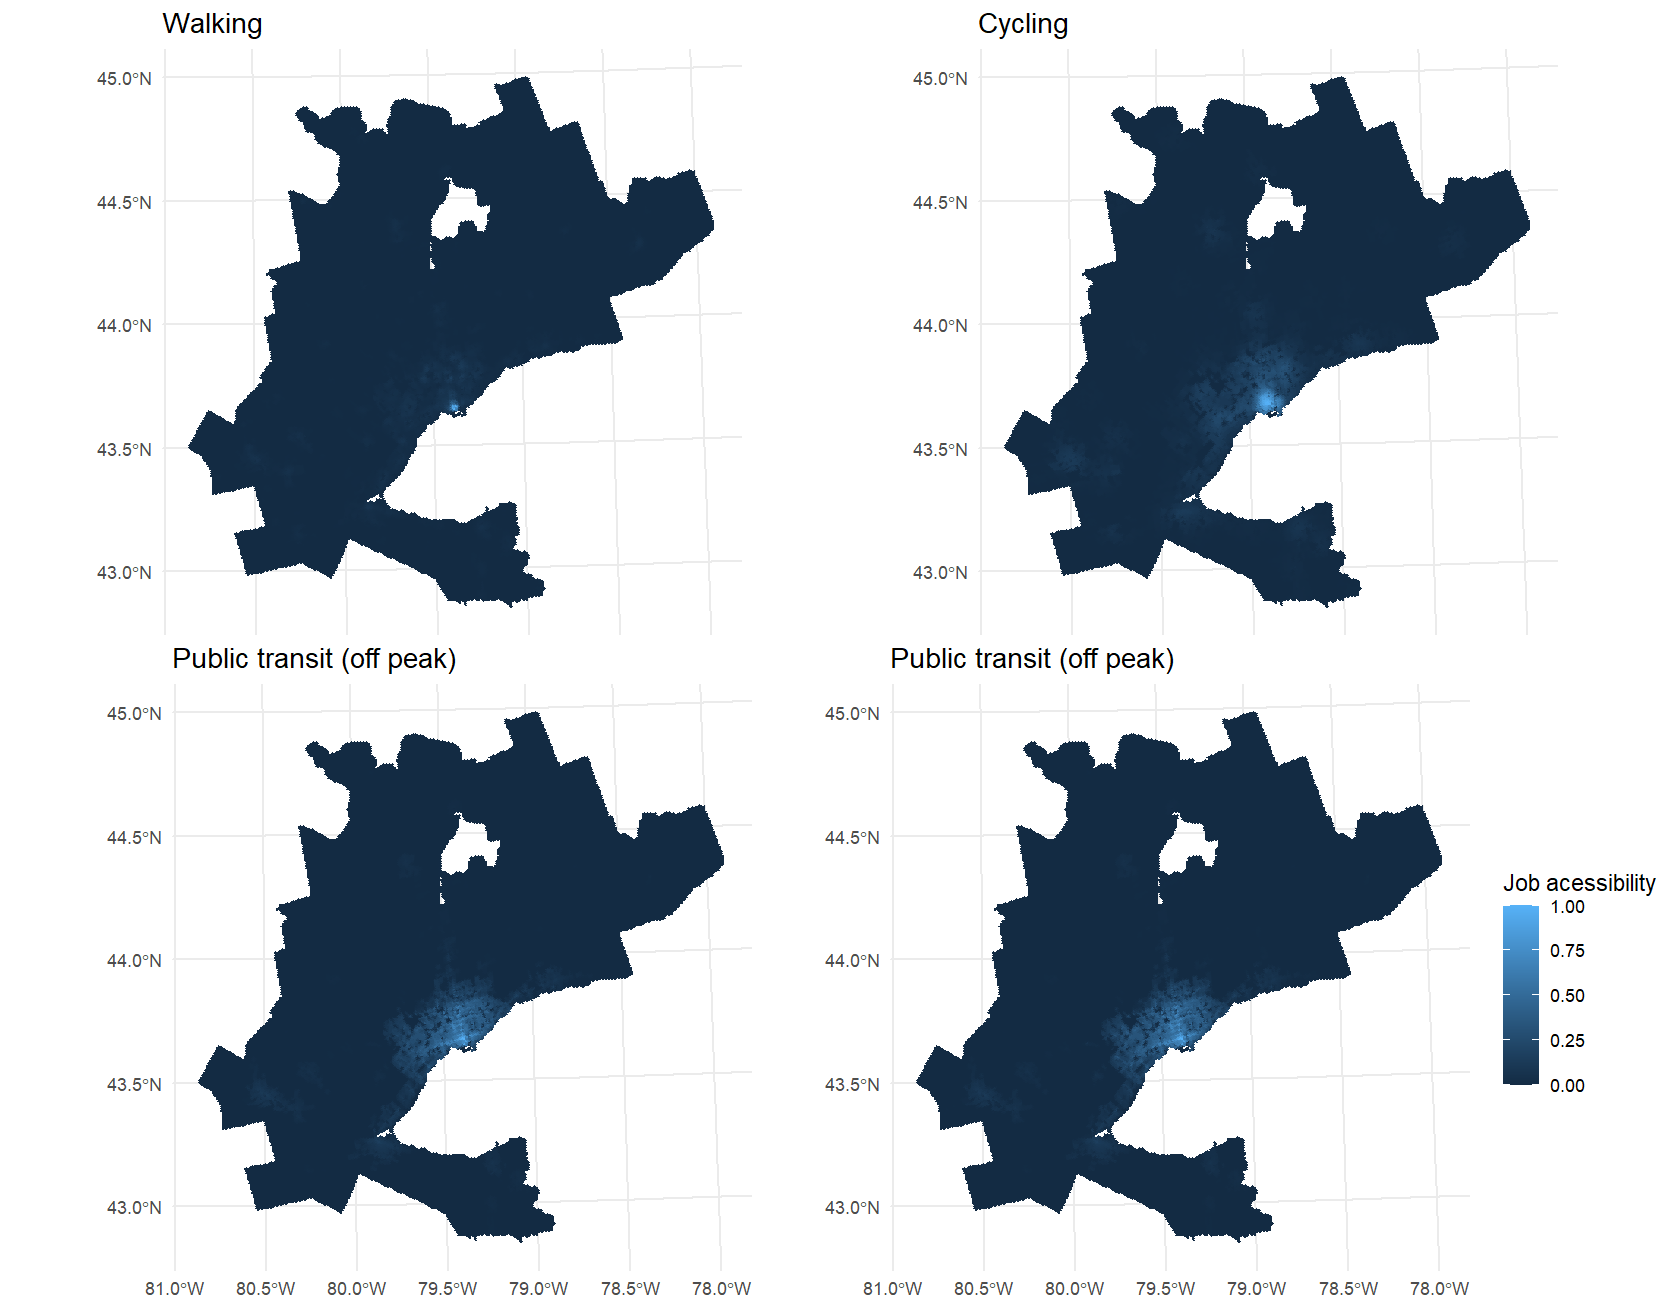
\includegraphics[width=3.5in]{C:/Users/brdia/Desktop/RSAccess/figures/job-access.png}
\caption{Job accessibility by mode in the Greater Golden Horseshoe Study Area.}
\label{fig:map_jobs}
\end{figure}

The spatial patterns exhibit differences in their median values of job
accessibility for all transportation modes: walking, cycling, public
transportation (off-peak), and public transportation (peak) (see Table
\ref{tab:tests_access}). The Kruskal-Wallis test results for all
transportation modes yield p-values \textless{} 2.2e-16, suggesting that
there is significant statistical evidence against the null hypothesis of
no difference in job accessibility between spatial patterns in the GGH.

\begin{table}[!ht]
\centering
\caption{COMPARISIONS OF JOB ACCESSIBILITY BETWEEN SPATIAL PATTERNS.}
\label{tab:tests_access}
\resizebox{\columnwidth}{!}{%
\begin{tabular}{@{}lrr@{}}
\toprule
\textbf{Mode} &
  \multicolumn{1}{l}{\textbf{\begin{tabular}[c]{@{}l@{}}Statistically different\\ (Kruskal-Wallis test)\end{tabular}}} &
  \multicolumn{1}{l}{\textbf{\begin{tabular}[c]{@{}l@{}}No statistical difference\\ (Pairwise Wilcoxon)\end{tabular}}} \\ \midrule
Walking                                                                                     & 1, 2, 3    & 4 and 5; 5 and 6 \\
Cycling                                                                                     & 1, 2, 3, 6 & 4 and 5          \\
\begin{tabular}[c]{@{}l@{}}Public   transit (off peak)\\ Public transit (peak)\end{tabular} & 1, 3, 4, 5 & 2 and 6          \\ \bottomrule
\end{tabular}%
}
\end{table}

Additionally, we observed that the spatial patterns ``Cluster 1 - High
Building Density'' and ``Cluster 3 - Medium Building Density'' exhibit
statistical differences in terms of job accessibility compared to the
other clusters. ``Cluster 4 - Mixed Rural Use'' and ``Cluster 6 - Farms
and Rural Neighborhoods'' show no statistical difference for walking
when compared to ``Cluster 5 - Waterfront Housing''. Cluster 4 also
shows no statistical difference for cycling when compared to Cluster 5.
On the other hand, ``Cluster 2 - Tree-lined Neighborhoods'' and Cluster
6 show no statistical difference across both public transit modes
(off-peak and on-peak).

\hypertarget{conclusion}{%
\section{Conclusion}\label{conclusion}}

The main objective of this study was to analyze and compare the levels
of accessibility to work in various spatial patterns in the Greater
Golden Horseshoe (GGH) region in Ontario, Canada. The comparison
involved four modes of transportation: walking, cycling and public
transit during peak and off-peak hours.

Initially, we identified six distinct spatial patterns in the study
area, characterized by differences in building density, land use,
location and street layout. Our analysis revealed that accessibility to
work varies across the study area, with spatial patterns that exhibit
higher building density also demonstrating high values of accessibility
to work, regardless of the mode of transport considered.

Notably, the study area has a low overall density, with less than 25\%
of cells containing more than 10\% residential and/or commercial area.
In addition, accessibility to work is concentrated in approximately 45\%
of the area analyzed, which corresponds to around 10\% of the GGH. This
concentration represents a complex challenge for spatial planners, as
employment opportunities are confined to a small part of the territory.
This scenario can lead to housing shortages in urban areas and require
complex strategies to develop a transportation system capable of dealing
with these territorial differences.

\hypertarget{references}{%
\section*{References}\label{references}}
\addcontentsline{toc}{section}{References}

\hypertarget{refs}{}
\begin{CSLReferences}{1}{0}
\leavevmode\vadjust pre{\hypertarget{ref-buchhorn}{}}%
Buchhorn, M., Smets, B., Bertels, L., Roo, B.D., Lesiv, M., Tsendbazar,
N.-E., Herold, M., Fritz, S., n.d. Copernicus Global Land Service: Land
Cover 100m: collection 3: epoch 2018: Globe.
doi:\href{https://doi.org/10.5281/ZENODO.3518038}{10.5281/ZENODO.3518038}

\leavevmode\vadjust pre{\hypertarget{ref-dossantos2022}{}}%
Dos Santos, B.D., De Pinho, C.M.D., Oliveira, G.E.T., Korting, T.S.,
Escada, M.I.S., Amaral, S., 2022. Identifying Precarious Settlements and
Urban Fabric Typologies Based on GEOBIA and Data Mining in Brazilian
Amazon Cities. Remote Sensing 14, 704.
doi:\href{https://doi.org/10.3390/rs14030704}{10.3390/rs14030704}

\leavevmode\vadjust pre{\hypertarget{ref-europeancommission.jointresearchcentre.2023}{}}%
European Commission. Joint Research Centre., 2023.
\href{https://data.europa.eu/doi/10.2760/098587}{GHSL data package
2023.} Publications Office, LU.

\leavevmode\vadjust pre{\hypertarget{ref-ontario2020}{}}%
Ontario, 2020.
\href{http://www.ontario.ca/page/planning-transportation-greater-golden-horseshoe}{Planning
transportation for the Greater Golden Horseshoe \textbar{} ontario.ca}.

\leavevmode\vadjust pre{\hypertarget{ref-openstreetmap2023}{}}%
OpenStreetMap, 2023. \href{https://www.openstreetmap.org/}{OpenStreetMap
Dataset}.

\leavevmode\vadjust pre{\hypertarget{ref-puxe1ez2012}{}}%
Páez, A., Scott, D.M., Morency, C., 2012. Measuring accessibility:
Positive and normative implementations of various accessibility
indicators. Journal of Transport Geography, Special section on
accessibility and socio-economic activities: Methodological and
empirical aspects 25, 141--153.
doi:\href{https://doi.org/10.1016/j.jtrangeo.2012.03.016}{10.1016/j.jtrangeo.2012.03.016}

\leavevmode\vadjust pre{\hypertarget{ref-palm2023}{}}%
Palm, M., Teel, S., Tiznado-Aitken, I., Soukhov, A., Paez, A., Farber,
S., Hain, M., 2023.
\href{https://mobilizingjustice.ca/wp-content/uploads/2023/06/Developing_Data_Driven_Standards_FINAL_2023_06_06.pdf}{Developing
data driven equity standards: Stakeholder perspectives}.

\leavevmode\vadjust pre{\hypertarget{ref-ringnuxe9r2008}{}}%
Ringnér, M., 2008. What is principal component analysis? Nature
Biotechnology 26, 303--304.
doi:\href{https://doi.org/10.1038/nbt0308-303}{10.1038/nbt0308-303}

\leavevmode\vadjust pre{\hypertarget{ref-statisticscanada}{}}%
Statistics Canada, n.d. Spatial Access Measures.

\end{CSLReferences}

\end{document}

